% THIS IS SIGPROC-SP.TEX - VERSION 3.1
% WORKS WITH V3.2SP OF ACM_PROC_ARTICLE-SP.CLS
% APRIL 2009
%
% It is an example file showing how to use the 'acm_proc_article-sp.cls' V3.2SP
% LaTeX2e document class file for Conference Proceedings submissions.
% ----------------------------------------------------------------------------------------------------------------
% This .tex file (and associated .cls V3.2SP) *DOES NOT* produce:
%       1) The Permission Statement
%       2) The Conference (location) Info information
%       3) The Copyright Line with ACM data
%       4) Page numbering
% ---------------------------------------------------------------------------------------------------------------
% It is an example which *does* use the .bib file (from which the .bbl file
% is produced).
% REMEMBER HOWEVER: After having produced the .bbl file,
% and prior to final submission,
% you need to 'insert'  your .bbl file into your source .tex file so as to provide
% ONE 'self-contained' source file.
%
% Questions regarding SIGS should be sent to
% Adrienne Griscti ---> griscti@acm.org
%
% Questions/suggestions regarding the guidelines, .tex and .cls files, etc. to
% Gerald Murray ---> murray@hq.acm.org
%
% For tracking purposes - this is V3.1SP - APRIL 2009

\documentclass{edm_template}
\usepackage{multirow}
\begin{document}

\title{YouEDU: Addressing Confusion in MOOC Discussion Forums by Recommending Instructional Video Clips}
%\subtitle{[Extended Abstract]
%\titlenote{A full version of this paper is available as
%\textit{Author's Guide to Preparing ACM SIG Proceedings Using
%\LaTeX$2_\epsilon$\ and BibTeX} at
%\texttt{www.acm.org/eaddress.htm}}}
%
% You need the command \numberofauthors to handle the 'placement
% and alignment' of the authors beneath the title.
%
% For aesthetic reasons, we recommend 'three authors at a time'
% i.e. three 'name/affiliation blocks' be placed beneath the title.
%
% NOTE: You are NOT restricted in how many 'rows' of
% "name/affiliations" may appear. We just ask that you restrict
% the number of 'columns' to three.
%
% Because of the available 'opening page real-estate'
% we ask you to refrain from putting more than six authors
% (two rows with three columns) beneath the article title.
% More than six makes the first-page appear very cluttered indeed.
%
% Use the \alignauthor commands to handle the names
% and affiliations for an 'aesthetic maximum' of six authors.
% Add names, affiliations, addresses for
% the seventh etc. author(s) as the argument for the
% \additionalauthors command.
% These 'additional authors' will be output/set for you
% without further effort on your part as the last section in
% the body of your article BEFORE References or any Appendices.

\numberofauthors{3} %  in this sample file, there are a *total*
% of EIGHT authors. SIX appear on the 'first-page' (for formatting
% reasons) and the remaining two appear in the \additionalauthors section.
%
\author{
% You can go ahead and credit any number of authors here,
% e.g. one 'row of three' or two rows (consisting of one row of three
% and a second row of one, two or three).
%
% The command \alignauthor (no curly braces needed) should
% precede each author name, affiliation/snail-mail address and
% e-mail address. Additionally, tag each line of
% affiliation/address with \affaddr, and tag the
% e-mail address with \email.
%
% 1st. author
\alignauthor Akshay Agrawal\\
       \affaddr{Stanford University}\\
       \email{akshayka@cs.stanford.edu}
% 2nd. author
\alignauthor Jagadish Venkatraman\\
       \affaddr{Stanford University}\\
       \email{vjagadish@cs.stanford.edu}
% 3rd. author
\alignauthor Andreas Paepcke\\
       \affaddr{Stanford University}\\
       \email{paepcke@cs.stanford.edu}
% \and   use '\and' if you need 'another row' of author names
}
\date{9 February 2015}
% Just remember to make sure that the TOTAL number of authors
% is the number that will appear on the first page PLUS the
% number that will appear in the \additionalauthors section.

\maketitle
\begin{abstract}
In Massive Open Online Courses (MOOCs), struggling learners often seek help by
posting questions in discussion forums. Unfortunately, given the large volume of discussion in MOOCs, instructors may overlook these learners' posts,
detrimentally impacting the learning process and exacerbating attrition. In this paper, we present YouEDU, an instructional aid that automatically detects and addresses confusion in forum posts. Leveraging our publicly-available Stanford MOOCPosts corpus, we train a heterogeneous set of classifiers to classify forum posts across multiple dimensions. In particular, classifiers that target sentiment, urgency, and other descriptive variables inform a single classifier that detects confusion. We then employ information retrieval techniques to map confused posts to minute-resolution clips from course videos; the ranking over these clips accounts for both video-clickstream data and textual similarity between posts and closed captions. We measure the performance of our classification model in multiple educational contexts, exploring the nature of confusion within each; we also evaluate the relevancy of materials returned by our ranking algorithm.
\end{abstract}

%% A category with the (minimum) three required fields
%\category{H.4}{Information Systems Applications}{Miscellaneous}
%%A category including the fourth, optional field follows...
%\category{D.2.8}{Software Engineering}{Metrics}[complexity measures, performance measures]
%
%\terms{Theory}

\keywords{ACM proceedings, \LaTeX, text tagging} % NOT required for Proceedings

\section{Introduction}
* Proliferation of MOOCs\\
* Volume of posts high\\
* Difficult to get a birds-eye view of the course, difficult to address it.\\

* Work looking into sentiment thus far is limited by datasets\\
* Work has been done on confusion, but not so much on MOOCs (save Rosé)\\
* Work into intelligently intervening + aiding the instructor\\
* Previous work has found forum to perhaps not be the most useful, even\\
* We suspect that the forum's perceived lack of usefulness is not instrinsic but rather ~ lack of attention lack of instructor tools + isolation from other parts of the classroom.\\
* We accordingly set out to adress both of these problems -- mining for affect gives instructors a pulse on the state of the course, and linking to videos marries forum and other course resources.\\
* Why video snippets as opposed to videos? \cite{Guo:2014:VPA:2556325.2566239} -- in a retrospective study of four edX courses, the maximum median engagement, regardless of video length, was six minutes.
* open sourced our entire implementation

The remainder of this paper is organized as follows. We examine related work in section two, present the Stanford MOOCPosts corpus in section three, sketch the architecture of YouEDU in section four, detail YouEDU's constituent classification and recommendation phases, evaluating both and interpreting results in sections five and six, and propose future work in section seven.

\section{Related Work}

\section{The Stanford MOOCPosts Corpus}
A precondition to automatically detecting affect in MOOC discussion forums was manually identifying it; given that no publicly-available corpus of tagged MOOC discussion forum posts existed prior to our research, we set out to create our own. The outcome of our data compilation and curation was the Stanford MOOCPosts dataset: a corpus composed of 29,604 anonymized learner forum posts from eleven Stanford University public online classes. Freely available to academic researchers, the MOOCPosts dataset was designed to enable computational inquiries into the nature of both affect and content in MOOC discussion forums.

Each post in the MOOCPosts dataset was scored across six dimensions -- confusion, sentiment, urgency, question, answer, and opinion -- and subsequently augmented with additional metadata. In this section, we detail the data collection methodology, defining each of the six dimensions along the way, and briefly present some insights gleaned by mining the set.


\subsection{Methodology: Compiling the Dataset}
Nine judges from oDesk were hired to ...

\subsection{Insights and Discussion}
We report insights gleaned into the nature of affect, etc. across these courses.

% TODO: Is this really the right place to present this? Or should this
% be presented in the Classification Combination Section?
\subsubsection{Relationship between Variables}
In this section, we report the pairwise correlations between variables to 1) shed some light into the nature of each and also 2) to motivate a YouEDU design choice.

% TODO: Perhaps fold this into the introduction.
\section{YouEDU: Detect and Recommend}

%TODO: Display + Caption
YouEDU is a personalized intervention system that recommends educational video clips to learners. Figure \ref{figure:architecture} illustrates the key steps that comprise YouEDU. YouEDU takes as input a set $P$ of forum posts, processing them in two distinct phases: (I) detection and (II) recommendation. In the first phase, we apply a classifier to each post in $P$, outputting a subset $P_{c}$ consisting of posts in which the classifier detected confusion. The confusion classifier functions as a \emph{combination} classifier in that it combines the predictions from classifiers trained to predict other post-related qualities.

\begin{figure}[ht]
       \centering
       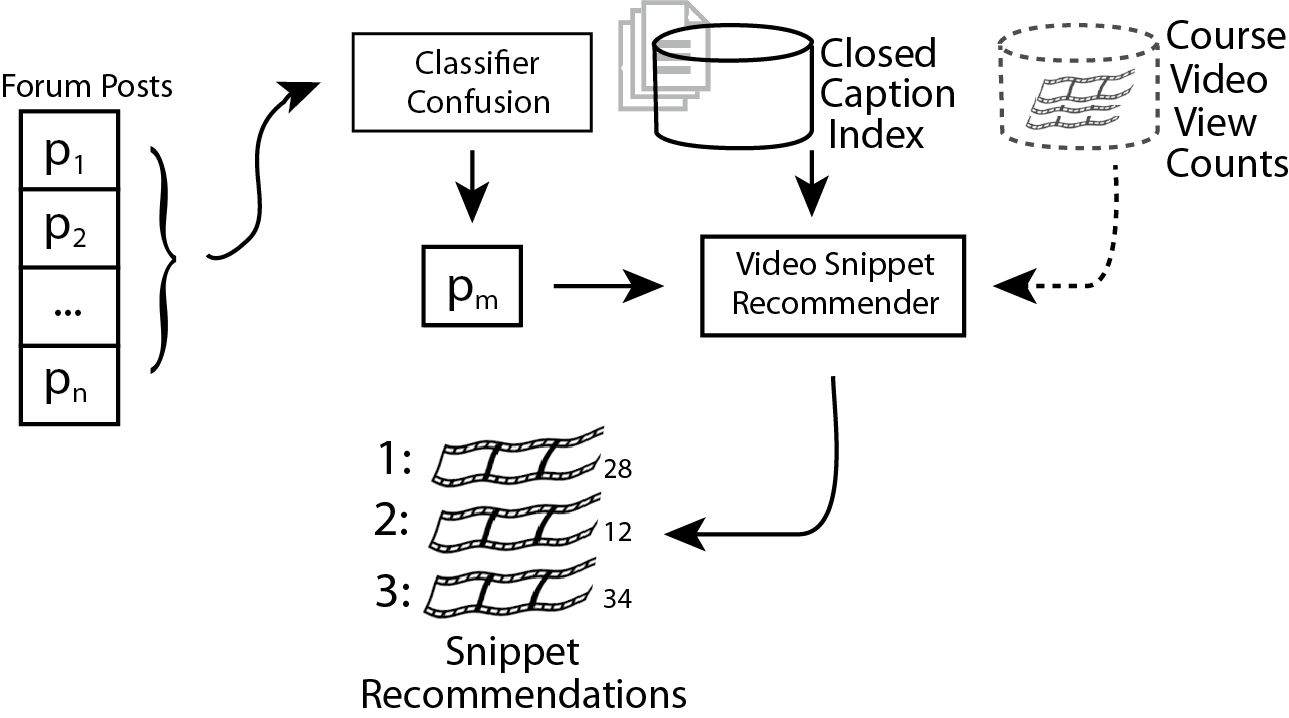
\includegraphics[width=0.5\textwidth]{../Figs/youEduArch.png}
       \caption{\textnormal{YouEDU Architecture. The YouEDU pipeline consists of two phases: post classification and video snippet recommendation.}}
       \label{figure:architecture}
\end{figure}

The second phase takes $P_{c}$ as input and, for each confused post in $p \in P_{c}$, outputs a ranked list of educational video snippets that address the object of confusion expressed in $p$. In particular, for a given post, the recommender produces an initial ranking across a number of one-minute video clips by computing a similarity metric between the post and closed caption sections. The ranking of videos in the retrieved set is then further informed by video-clickstream data.

While YouEDU outputs minute-resolution video clips, it does not necessarily guarantee that these clips fully address the exhibited confusion -- indeed, several minutes of instructional content are often required to explain a single concept. Rather, the video snippets collectively form an ad-hoc index. For example, say that for a given post, YouEDU outputs three video snippets with start times $s_{1}, s_{2}, s_{3}$, in order of decreasing relevance, and say that these snippets were contained in videos $v_{1}, v_{2}, v_{3}$, respectively, $v_{1}, v_{2}, v_{3}$ not necessarily unique. In order to clarify his or her confusion, the author of the post should begin watching video $v_{1}$ at $s_{1}$ -- the learner can autonomously set the end time of the snippet, and can move on to the next video, start time pair if any confusion still lingers. 

In the following two sections, we delve further into both phases of YouEDU, describing them in detail and relating the results of empirical evaluations.

\section{Phase I: Detecting Confusion}
% TODO: Cite
We frame the problem of detecting confusion as a binary one: Given a discussion forum post $p$ with a true label $L$ in \{not confused, confused\}, apply some hypothesis $h$ that correctly divines $L$. Posts with a confusion rating greater than four in the MOOCPosts dataset fall into the ``confused'' class, while all other posts fall into the ``not confused'' class.

We craft a rich feature space that fully utilizes the data available in our MOOCPosts dataset, choosing logistic regression with $l_{2}$ regularization as our statistical model. Results from empirical evaluations demonstrate that our classifier performs reasonably well, while simultaneously providing insight into the nature of confusion across multiple courses.

\subsection{Feature Space and Model Design}
Our feature space is composed of three types of inputs, those derived from: the post body; post metadata; and other classifiers. The confusion classifer we train functions as a combining layer that folds in the predictions of other classifiers; these classifiers are trained to predict variables correlated with confusion. We expand upon each type of input here.

\subsubsection{Bag-of-Words}
We take the bag-of-words approach in representing documents, or forum posts. Each document is represented in part as a vector of indicator variables, one for each word that appears in the training data -- the $i$-th indicator is one if the $i$-th word in the vocabulary is present in the document, zero otherwise. A word is defined as either a sequence of one or more alphanumeric characters or a single punctuation character (one of \{. , ; ! ?\}).

Documents are pre-processed before they are mapped to vectors. We prune out stop words, using a subset of the stop word list published by the Information Retrieval Group at the University of Glasgow \cite{glasgow}. Removed words inlcude, but are not limited to, interrogatives (``who'', ``what'', ``where'', ``when'', ``why'', ``how''), words that identify the self (``I'', ``my''), verbs indicating ability or the lack thereof, negative words (``cant'', ``cannot'', ``couldnt''), and certain conjunctions (``yet'', ``but''). We ignore alphabetic case\footnote{All-caps discussion certainly does communicate affect in some Internet forums -- it is typically associated with aggression and is considered a breach of ``nettiquette'' \cite{hambridge1995netiquette}; however, we assume that MOOC forum-goers are somewhat civil, and so accounting for case would needlessly inflate our feature space.} and lemmatize numbers, \LaTeX\ equations, and URLs. Intuitively, the presence of numbers and equations in a forum post might indirectly convey confusion or the lack thereof, in that the learner may be asking a question about some quantity or perhaps providing an answer to a quantitative question; similarly, a knowledgeable learner might answer a question by citing a URL. 

The unigram document representation, while simple, pervades text classification and often achieves high performance \cite{boulis2005text}. We employ $l_{2}$ regularization in order to prevent overfitting, a risk that is aggravated when the dimension of the feature space exceeds the training set size \cite{Ng:2004:FSL:1015330.1015435}.

\subsubsection{Post Metadata}
The feature vector derived from unigrams is augmented with post metadata, including: 
\vspace{-15pt}
\begin{itemize}
       \item The number of up-votes accumulated by the post. We rationalized that learners might express interest in posts that voiced confusion that they shared. 
       \item The number of reads garnered by the post's containing thread.
       \item Whether the poster elected to appear anonymous to his or her peers or to the entire population. It has been shown that anonymity in educational discussion forums enables learners to ask questions without fear of judgement \cite{freeman2004student}, and our dataset demonstrates a strong correlation between questions and confusion.
       \item The post author's grade in the class at the time of post submission, where ``grade'' is defined as the numer of points earned by the learner (e.g., by correctly answering quiz questions) divided by the number of points possible. The lower the grade, we hypothesized, the more likely the student might be confused about a topic.
\end{itemize}

\subsubsection{Classifier Combination}
In section 3.2, we demonstrated that, at least in the humanities and medicine courses, confusion is significantly correlated with questions, answers, urgency, sentiment and opinion. As such, in predicting confusion, we take into account the predictions of five distinct classifiers, one for each of the aforementioned variables. We use the fine-grained method of combining classifiers in which the outputs of several classifiers are fed as input to a \emph{combination function} \cite{bennett2005combination}. In our case, the combination function is itself a classifier.

For a given train-test partition, let $D_{train}$ be the training set and $D_{test}$ be the test set. In both sets, each example is tagged along the six variables. Let $H_{q}$, $H_{a}$, $H_{o}$, $H_{s}$, and $H_{u}$ be classifiers for the question, answer, opinion, sentiment, and urgency variables, respectively. We call these classifiers \emph{constituent} classifiers. Each constituent is trained on $D_{train}$, taking as input bag-of-words and post metadata features, as described in the previous two subsections. 

Let $H_{c}$, a classifier for confusion, be our combination function. Like the constituent classifiers, $H_{c}$ is trained on $D_{train}$ and takes as input bag-of-words and metadata features. Unlike the constituents, $H_{c}$ also treats the ground-truth labels for the question, answer, opinion, sentiment, and urgency variables as features. When testing $H_{c}$ on an example $d \in D_{test}$, the constituent classifiers each output a prediction for $d$. These five predictions are appended to the bag-of-words and metadata features derived from $d$. The resulting vector is given as input to $H_{c}$, which then predicts $d$'s confusion class.

A few subtleties: $H_{s}$ uses an additional metadata feature that the other classifiers do not -- the number of negative words (e.g., ``not'', ``cannot'', ``never'', etc.). $H_{q}$, $H_{a}$, $H_{u}$, and $H_{c}$ treat the number of question marks as an additional feature, given the previously presented correlations; \cite{wen2015confusion} also used question marks in predicting confusion. And while $H_{q}$, $H_{a}$, and $H_{o}$ are by nature binary classifiers, $H_{s}$ and $H_{u}$ are multi-class. The latter three predict values in $\{ 1 + 0.5x \mid x \le 12 \}$. By preserving the full range, we provide $H_{c}$ with granular information about the non-confusion variables.

\subsection{Evaluation}
For clarity, we refer to the confusion classifier that uses all the features described in the section 5.1 as the \emph{complete} classifier. In this section, we evaluate and interpret the performance of both the complete classifier and confusion classifiers with pared-down feature sets, reporting insights and intuitions gleaned about the nature of confusion in MOOCs along the way. 

The complete classifier was evaluated in three contexts: course sets, individual courses, and across courses. In each context, we attempted the binary classification problem defined in the previous subsection. In the former two contexts, we report the average performance of 10-fold stratified cross validation (the nature of training and testing across courses, explained further below, does not allow for cross validation). We quantify performance using two metrics: $F_{1}$ and Cohen's Kappa. 

\begin{table*}
    \centering
    \begin{tabular}{|c|c c c|c c c|c|}
    \hline
    \multirow{2}{*}{Course Set} & \multicolumn{3}{c|}{Not Confused} & \multicolumn{3}{c|}{Confused}  & \multirow{2}{*}{Kappa} \\ \cline{2-7}
                                &  Precision & Recall & $F_{1}$     &  Precision & Recall & $F_{1}$  &       \\ \hline
    Humanities                  & 0.898      & 0.943    & 0.919     & 0.778      & 0.642  & 0.700    & 0.621  \\ \hline
    Medicine                    & 0.924      & 0.946    & 0.935     & 0.699      & 0.589  & 0.627    & 0.564  \\ \hline

    \end{tabular}
    \caption{\textnormal{
       Complete Confusion Classifier Performance, Course Sets. For each course set listed, this table reports the average performance across 10 folds of stratified cross validation.
    }} % title of Table
    \label{table:confusion_sets} % is used to refer this table in the text
\end{table*}

\begin{table*}
       \centering
       \begin{tabular}{|c|c|c|c|}
       \hline
       Course                         & $F_{1}$: Not Confused & $F_{1}$: Confused & Kappa \\ \hline
       Managing Emergencies           & 0.963                 & 0.771             & 0.741 \\ \hline
       Statistical Learning           & 0.909                 & 0.767             & 0.677 \\ \hline
       Economics 1                    & 0.933                 & 0.741             & 0.675 \\ \hline
       Statistics in Medicine (2014)  & 0.908                 & 0.748             & 0.658 \\ \hline
       Statistics in Medicine (2013)  & 0.916                 & 0.671             & 0.589 \\ \hline
       Science Writing                & 0.961                 & 0.527             & 0.491 \\ \hline
       Women's Health                 & 0.933                 & 0.506             & 0.445 \\ \hline
       How to Learn Math              & 0.970                 & 0.383             & 0.389 \\ \hline
       \end{tabular}
       \caption{\textnormal{
       Complete Confusion Classifier Performance, Individual Courses. Our classifier performed best on courses whose discourse was characterized by technical diction, like statistics or economics. In courses like \emph{How to Learn Math} that facilitated open-ended and somewhat roaming discussions, our model found it more difficult to implicitly define confusion. 
       }} % title of Table
       \label{table:confusion_courses} % is used to refer this table in the text
\end{table*}


\begin{table}
       \centering
       \begin{tabular}{|c|c|c|}
       \hline
       Training Course                & Test Course                    & Kappa \\ \hline
       Statistics in Medicine (2013)  & Statistics in Medicine (2014)  & 0.629 \\ \hline
       Statistical Learning           & Statistics 216                 & 0.590 \\ \hline
       Economics 1                    & Statistics in Medicine (2013)  & 0.267 \\ \hline
       Women's Health                 & Statistics in Medicine (2013)  & 0.264 \\ \hline
       Statistics in Medicine (2013)  & Women's Health                 & 0.175 \\ \hline
       \end{tabular}
       \caption{\textnormal{
       Nature of Confusion Across Domains. Training and testing on similar courses typically resulted in high performance, especially in the case of technical courses. The low score associated with training on Statistics in Medicine and testing on Women's Health suggests that the nature of confusion in the former is particularly related to domain concepts.
       }} % title of Table
       \label{table:across_courses} % is used to refer this table in the text
\end{table}


* educational contexts \\
* metrics used \\ 
* results \\
* implications \\

\section{Phase II: Recommending Clips}
\subsection{The Recommendation Algorithm}
\subsubsection{Retrieval}
\subsubsection{Ranking}

\subsection{Evaluation}
Two experts were hired ...

\section{Future Work}
Future work might focus on strengthening the link between the classifiers and the reccomendation system; in particular, it would behoove us to devise a way to filter our set of confused posts to a subset for which recommendation makes sense. Additionally, we might want to make our classifiers better and index back into the previous course to retrieve answers for courses. Deploying this system live is another thing that we might do. 

YouEDU's two phases need not be packaged together; in an online setting, they could operate as independent, complemetary services. The output of Phase I could be presented directly to instructors, many of whom express interest in understanding activity in discussion forums \cite{Stephens-Martinez:2014:MMI:2556325.2566246}. As for Phase II, the recommendation system might live as a search-box of sorts: learner would type natural language queries in which they voiced their confusion, and our system would serve them relevant resources.

\section{Conclusion}
YouEDU takes an initial step towards building automated confusion intervention ... 

%\end{document}  % This is where a 'short' article might terminate

%ACKNOWLEDGMENTS are optional
\section{Acknowledgments}
This section is optional\cite{wen2014sentiment}; it is a location for you
to acknowledge grants, funding, editing assistance and
what have you.  In the present case, for example, the
authors would like to thank Gerald Murray of ACM for
his help in codifying this \textit{Author's Guide}
and the \textbf{.cls} and \textbf{.tex} files that it describes.

%
% The following two commands are all you need in the
% initial runs of your .tex file to
% produce the bibliography for the citations in your paper.
\bibliographystyle{abbrv}
\bibliography{sources}  % sigproc.bib is the name of the Bibliography in this case
% You must have a proper ".bib" file
%  and remember to run:
% latex bibtex latex latex
% to resolve all references
%
% ACM needs 'a single self-contained file'!
%
%APPENDICES are optional
%\balancecolumns
\balancecolumns
% That's all folks!
\end{document}
